\begin{ex}
(Ufla-MG) Em um programa de auditório, utiliza-se uma roleta como na figura:
 \begin{center}
     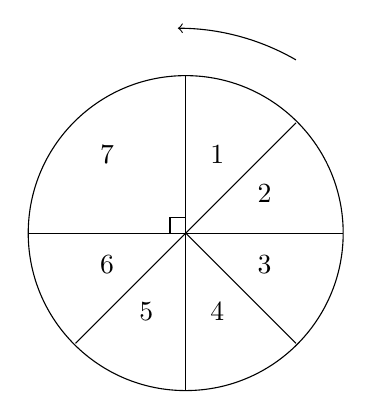
\begin{tikzpicture}
      \draw (0,0) circle [radius = 2];
      \draw (-2,0)--(2,0); \draw (0,-2)--((0,2);
      \draw (-1.4,-1.4)--(1.4,1.4);
      \draw (0,0)--(1.4,-1.4); 
      \draw (-.2,0)--(-.2,.2);
      \draw (0,.2)--(-.2,.2);
      \node at (-1,1) {7}; \node at (1,.5) {2};
      \node at (.4,1) {1};\node at (.4,-1) {4};
      \node at (1,-.4) {3};\node at (-.5,-1) {5};
      \node at (-1,-.4) {6};
      \draw [->] (1.4,2.2) arc [radius=3, start angle=60, end angle = 90];
     \end{tikzpicture}
 \end{center}


Os ângulos de 1 a 6 são iguais. A roleta é girada 3 vezes. Calcule a probabilidade de os números obtidos no primeiro giro, no segundo giro e no terceiro giro serem respectivamente, 1, 2 e 3.
 \begin{sol}
   \phantom{A} \\
   a roleta tem 8 ângulos de $45^{\circ} \Longrightarrow p= \frac{1}{8}\cdot \frac{1}{8}\cdot \frac{1}{8}=\frac{1}{512}$ 
 \end{sol}
\end{ex}